\documentclass[line,margin]{res} 

\usepackage{tikz}

\begin{document}
	\name{David S. McDermott}
	\address{235 S. Buckhout St. State College, PA 16801}
	\address{(484) 904-2099}
	
	\begin{resume}
		\section{HIGHLIGHTS} Dual major student at Penn State with concentrations in computer architecture and solid state engineering with research experience in semiconductor fabrication process and design for test methodologies.  Previously worked at Penn State ARL developing intelligence applications for data ingest and visualization resulting in an active US Secret clearance and at IBM developing Logic Built in Self Test (LBIST) routines for Z series processors on a new test platform with a flexible object oriented interface.
		
		\section{SKILLS}
		\textbf{Programming Languages:} Java, C, C++, C\#, x86 Assembly, MIPS Assembly\\
		\textbf{Scripting Languages:} Python, MATLAB, Shell (Bash), Perl, PHP, Batch\\
		\textbf{Design Tools:} Cadence Virtuoso, Autodesk EAGLE, KiCAD, NI Multisim
		
		\section{EDUCATION}{\sl Bachelor of Science} Computer Engineering, Electrical Engineering \\
		The Pennsylvania State University, University Park, PA \hfill May 2019\\
		College of Engineering \& Schreyer Honors College\\
		Majors: Computer Engineering, Electrical Engineering \hfill GPA: 3.53/4.00
		
		\section{EXPERIENCE}{\sl Design for Test and Characterization Intern} \hfill May 2018 - Present\\
		IBM, z/Systems, Poughkeepsie, NY
		\begin{itemize}  \itemsep -2pt
			\item Assisted in migration from single use Perl scripts to object oriented Python
			\item Assisted in development of new chip test platform based on Kintex Ultrascale
			\item Developed CP Logic Built in Self Test routines that ran 40\% faster than before
			\item Developed interactive testing and visualization platform for characterization
			\item Identified potential 10\% reduction in dynamic power of latches for z/CP
			\vspace*{-\baselineskip}		
		\end{itemize}
		\textbf{Relevant Skills:} Python, Jupyter, SQL, Neo4j, Cypher Query, VLSI, VHDL, BIST
		
		{\sl Visualization Intern} \hfill May 2017 - May 2018 \\
		The Pennsylvania State University ARL, SEALab, University Park, PA
		\begin{itemize}  \itemsep -2pt
			\item Supported development for existing visualization applications in an Agile team
			\item Parallelized physics simulation and rendering engines on existing application
			\item Resolved race conditions in scene graph of rendering engine for CAVEs
			\item Developed several new data pipelines for databases, blockchains and Excel
			\vspace*{-\baselineskip}		
		\end{itemize}
		\textbf{Relevant Skills:} Java, OpenGL, C, SQL, SQLite, Apache Tomcat, Unity 3D, C\#
		\textbf{Other Information:} Active US Secret Clearance
		
		\section{Projects}	{\sl 4KB SRAM Cache} \hfill Fall 2018\\
		The Pennsylvania State University, CMPEN/EE 416
		\begin{itemize}  \itemsep -2pt
			\item Worked with partner to develop 4KB SRAM Cache using 200nm TSMC process
			\item Developed Python tools to optimize path length \& transistor sizing
			\item Completed schematic, layout, and simulation using HSPICE
			\vspace*{-\baselineskip}		
		\end{itemize}
		\textbf{Relevant Skills:} VLSI, Cadence Virtuoso, Computer Architecture, Python
		\begin{tikzpicture}[remember picture, overlay]
		%\node[xshift=-140mm, yshift=10mm]{%
		%	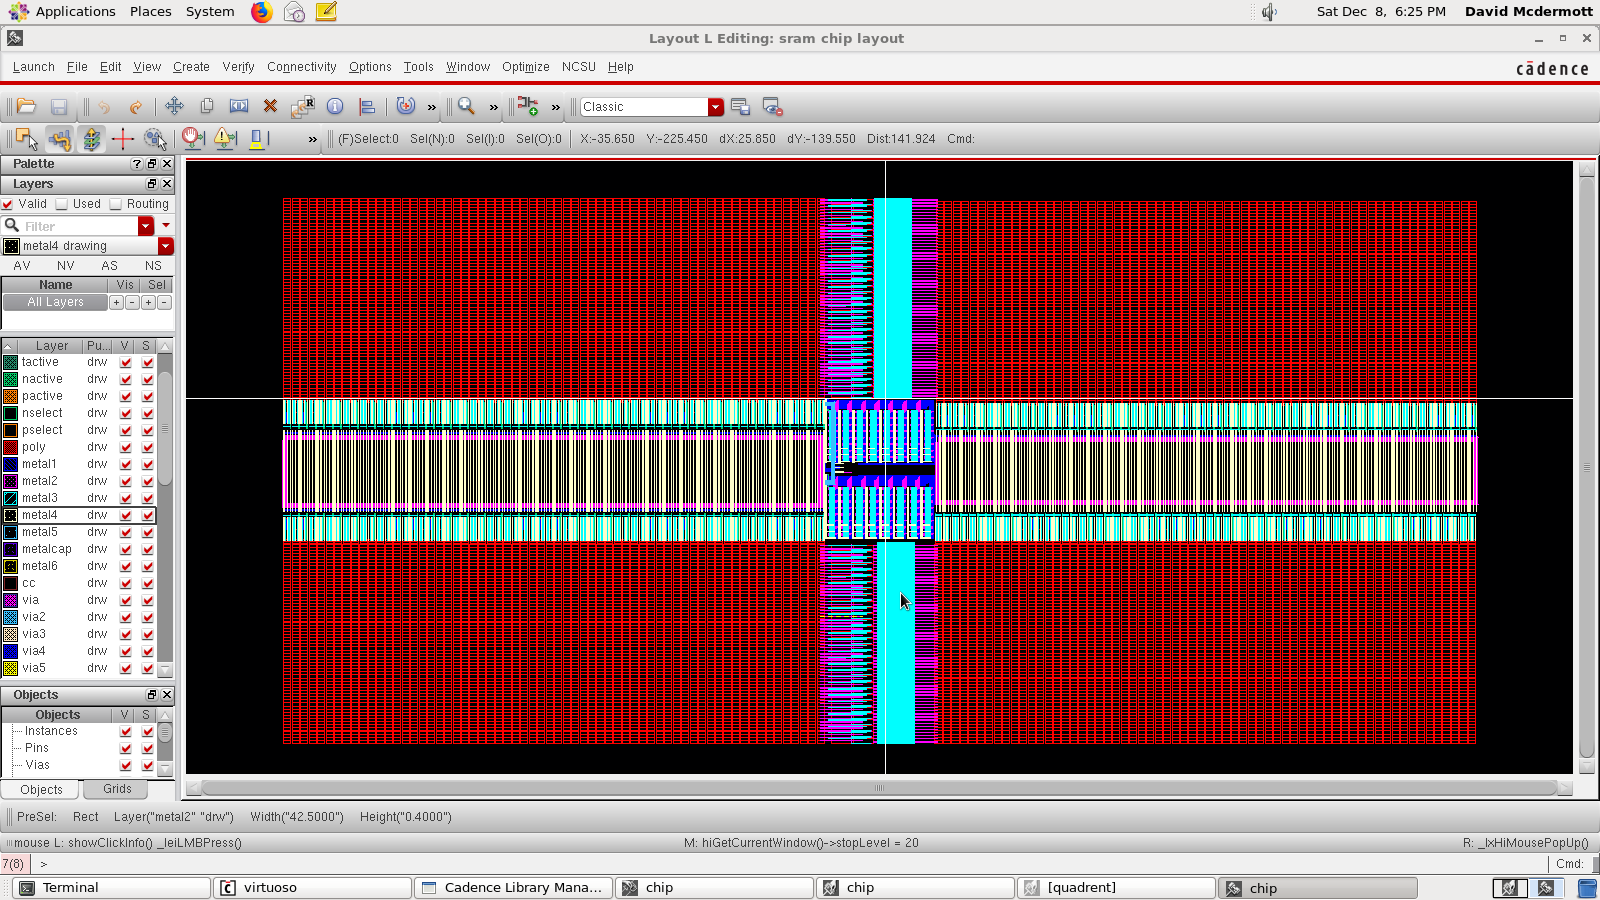
\includegraphics[width=35mm]{SRAM}};
		\end{tikzpicture}
		
		{\sl Wristband Scanner} \hfill Spring 2018 - Present\\
		The Pennsylvania State University, HackPSU
		\begin{itemize}  \itemsep -2pt
			\item Worked with a team of several other students to develop an IOT scanner
			\item Developed C++ abstractions for Arduino to interface with RFID scanner chips
			\item Developing PCB design with multiple micro-controllers and planar antennae
			\vspace*{-\baselineskip}		
		\end{itemize}
		\textbf{Relevant Skills:} C++, Arduino, PCB Design, Antenna Design
		\begin{tikzpicture}[remember picture, overlay]
		%\node[xshift=-122mm, yshift=10mm]{%
		%	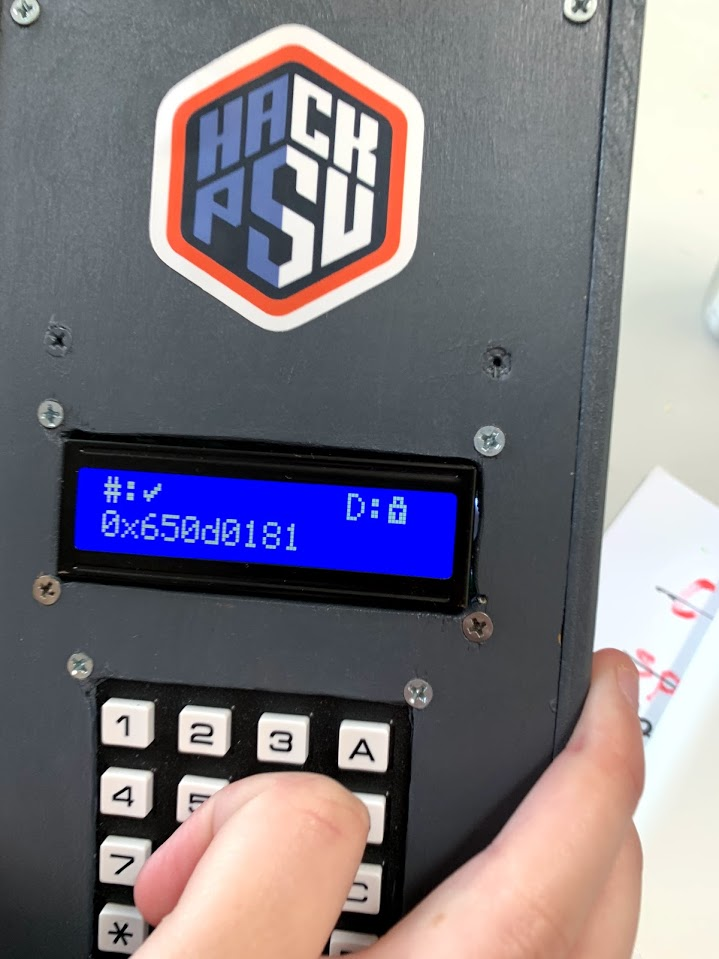
\includegraphics[height=35mm]{SCAN}};
		\end{tikzpicture}
	\end{resume}

\end{document}